%!TEX root=../main.tex
\section{Results}
We compare the performance of exact Gaussian processes against widely-used scalable GP approximation methods on a range of large-scale datasets from the UCI dataset repository \cite{asuncion2007uci}.
Our experiments demonstrate that exact GPs:
(1) outperform popular approximate GPs methods on nearly all benchmarking datasets in our study;
(2) compute thousands of test-point predictions in less than a second, even when $n > 10^6$;
(3) utilize all available data when making predictions, even when $n > 10^5$; and
(4) achieve linear training speedups on large datasets by adding additional GPU devices.

\paragraph{Baselines.}
We compare against two scalable GP approximations: Sparse Gaussian Process
Regression (SGPR) \cite{titsias2009variational,matthews2016scalable},
and Stochastic Variational Gaussian Processes (SVGP) \cite{hensman2013gaussian}.
We choose these methods due to their popularity and general applicability, enabling a comparison over a wide
range of datasets. SGPR is an inducing point method where the inducing points are learned through a variational objective.
We use $m = 512$ for SGPR and $m = 1,\!024$ for SVGP, which are common values used for these methods \cite{matthews2017gpflow}.
We later experiment with varying the number of inducing points.

\paragraph{Experiment details.}
We extend the \href{https://gpytorch.ai}{GPyTorch} library \cite{gardner2018gpytorch} to perform all experiments.
Each dataset is randomly split into $4/9$ training, $2/9$ validating, and $3/9$ testing sets. We use the validation set for tuning parameters like the CG training tolerance.
The data is whitened to be mean $0$ and standard deviation $1$ as measured by the training set.
We use a constant prior mean and a Mat\'ern 3/2 kernel with independent lengthscales for each dimension.

\begin{figure*}[h!]
  \centering
  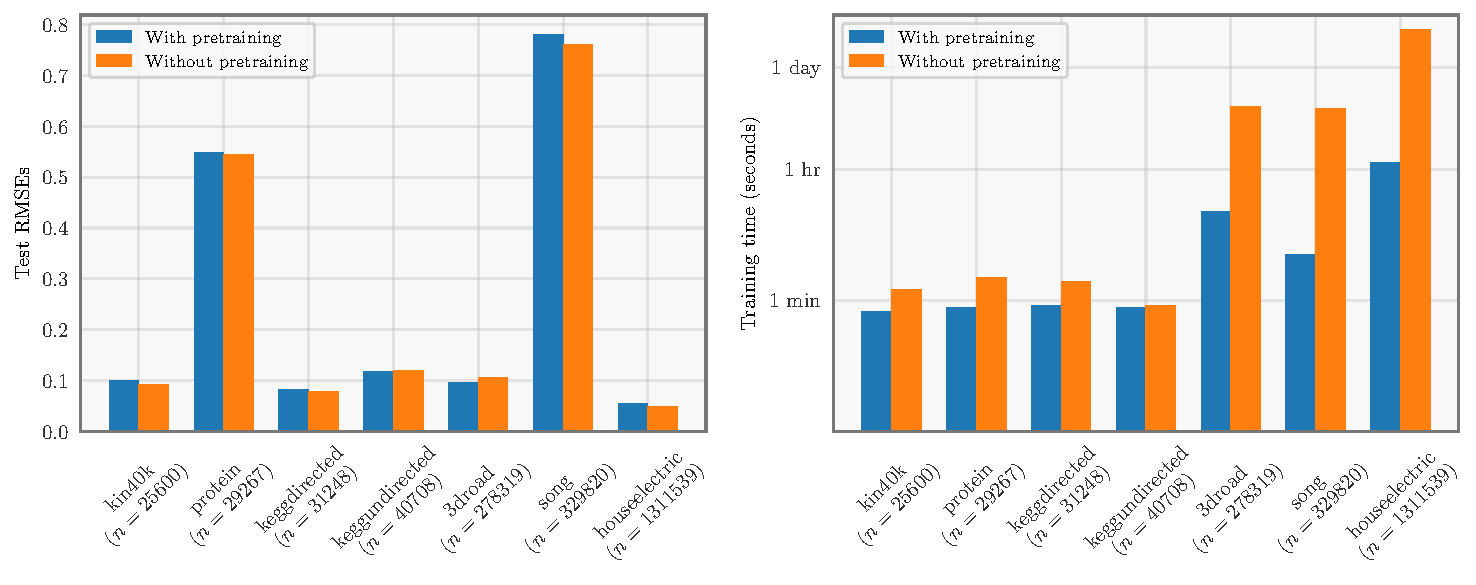
\includegraphics[width=\linewidth]{figures/initialization-rmse-timings.pdf}
  \caption{
	A comparison of exact GPs trained using our initialization procedure against exact GPs trained for 100 iterations using Adam.
	Better initializatoin allows exact GPs to achieve similar RMSEs while requiring drastically less training time on large datasets.
  }
  \label{fig:initialization-test}
\end{figure*}
We learn model hyperparameters and variational parameters
by optimizing the log marginal likelihood.
For SGPR, we perform $100$ iterations of Adam with a learning rate of $0.1$.
For SVGP, we perform $100$ epochs of Adam with a minibatch size of $1,\!024$ and a learning rate of $0.01$, which
we found to perform better than $0.1$.
\textit{For exact GPs, the number of optimization steps has the greatest
effect on the training time for large datasets.} To reduce the training time for
exact GPs, we first randomly
subset $10,\!000$ training points from the full training set to fit an exact GP whose hyperparameters will be used as initialization. We pretrain on this subset with 10 steps
of L-BFGS \citep{liu1989lbfgs} and 10 steps of Adam \citep{kingma2014adam} with $0.1$ step size before using the learned hyperaparameters to take 3 steps of Adam on the full training dataset. \autoref{fig:initialization-test} shows
that this initialization plus fine-tuning procedure achieves comparable test
performance to running Adam for the full 100 iterations without pretraining.
We do not pretrain the SGPR and SVGP models because we found that they
required a significant number of fine-tuning steps after pretraining due to
their increased number of model parameters. We show additional training
statistics for exact GPs trained with 100 steps of Adam in the appendix.

For all experiments, we use a rank-$100$ partial pivoted-Cholesky preconditioner and
run PCG with a tolerance of $\epsilon = 1$ during training.
We constrain the learned noise to be at least 0.1 to regularize the poorly
conditioned kernel matrix for the houseelectric dataset.
We perform all training on a single machine with 8 NVIDIA Tesla V100-SXM2-32GB-LS GPUs.
Code to reproduce the experiments is available at \url{https://gpytorch.ai}.
\begin{table*}[h!]
  \caption{
	  Root-mean-square-error (RMSE) and negative log-likelihood (NLL) of exact GPs and approximate GPs on UCI regression datasets using a constant prior mean and a Mat\'ern 3/2 kernel. All trials were averaged over 3 trials with different splits.  $\pm$ corresponds to 1 standard deviation.
    $n$ and $d$ are the size and dimensionality of the training dataset,
    respectively. The number of GPUs used and the number of kernel partions are reported in \autoref{tab:large_exact_gp_timings}.
    We were unable to scale SGPR to HouseElectric due to its memory requirements when $m=512$.
    \vspace{0.3em}
  }
  \label{tab:no_ard_rmse_nll}
  \centering
  \resizebox{\textwidth}{!}{%
    \begin{tabular}{ cccccc }
  \toprule
  &&&
	\multicolumn{3}{c}{{\bf RMSE}}  \\
  \cmidrule{4-6}
  \thead{\\{\bf Dataset}} & \thead{\\$N$} & \thead{\\$D$} &
  \thead{{\bf Exact GP} \\ (BBMM)} & \thead{{\bf SGPR} \\ ($M\!=\!512$)} & \thead{{\bf SVGP} \\ ($M\!=\!1,\!024$)}
  \\
  \midrule
	PoleTele             & $9,\!600$          & $26$  &   $\mathbf{0.151}\pm 0.012$  & $0.217\pm 0.002$          & $0.215\pm 0.002$  \\
	Elevators            & $10,\!623$         & $18$  &   $\mathbf{0.394}\pm 0.006$  & $0.437\pm 0.018$          & $0.399\pm 0.009$  \\
	Bike                 & $11,\!122$         & $17$  &   $\mathbf{0.220}\pm 0.002$  & $0.362\pm 0.004$          & $0.303\pm 0.004$  \\
	Kin40K               & $25,\!600$         & $8$   &   $\mathbf{0.099}\pm 0.001$  & $0.273\pm 0.025$          & $0.268\pm 0.022$  \\
	Protein              & $29,\!267$         & $9$   &   $\mathbf{0.536}\pm 0.012$  & $0.656\pm 0.010$          & $0.668\pm 0.005$  \\
	KeggDirected         & $31,\!248$         & $20$  &   $\mathbf{0.086}\pm 0.005$  & $0.104\pm 0.003$          & $0.096\pm 0.001$  \\
	CTslice              & $34,\!240$         & $385$ &   $0.262\pm 0.448$           & $\mathbf{0.218}\pm 0.011$ & $1.003\pm 0.005$  \\
	KEGGU                & $40,\!708$         & $27$  &   $\mathbf{0.118}\pm 0.000$  & $0.130\pm 0.001$          & $0.124\pm 0.002$  \\
	3DRoad               & $278,\!319$        & $3$   &   $\mathbf{0.101}\pm 0.007$  & $0.661\pm 0.010$          & $0.481\pm 0.002$  \\
	Song                 & $329,\!820$        & $90$  &   $0.807\pm 0.024$           & $\mathbf{0.803}\pm 0.002$ & $0.998\pm 0.000$  \\
  Buzz                 & $373,\!280$        & $77$  &   $\mathbf{0.288}\pm 0.018$  & $0.300\pm 0.004$          & $0.304\pm 0.012$  \\
	HouseElectric        & $1,\!311,\!539$    & $9$   &   $\mathbf{0.055}\pm 0.000$  & -----                     & $0.084\pm 0.005$  \\
  \bottomrule
\end{tabular}

  }
\end{table*}

\paragraph{Accuracy.}
\autoref{tab:no_ard_rmse_nll} displays the accuracy and negative log likelihoods of exact GPs and approximate methods on several large-scale datasets using independent lengthscale across dimensions.
We find that exact GPs achieve lower error than approximate methods on nearly every dataset. Notably, on certain datasets
like Kin40K and CTslice, exact GPs achieve a half or even a quarter of the error of some approximate methods, and consistently outperform
the approximate methods even on datasets with up to over 1M data points.
Although \citet{nguyen2019exact} show results for exact GPs on $n < 120,\!000$, this is the first set of results comparing exact GPs to approximate GPs on $n\gg 10^5$.

Interestingly, the size or the dimensionality of the dataset does not seem to influence the relative performance of the approximate methods.
For example, though Protein and Kin40K  are similar in size and have almost the same dimensionality, the approximate methods perform worse on Kin40K (relative to the RMSE of exact GPs).
Moreover, we also see that the choice of approximate method affects performance, with neither approximate method consistently outperforming the other.

\begin{table*}[t!]
  \caption{
    Timing results for training and prediction for exact GPs and approximate GPs.
    Training times were recorded using the same hardware and other experimental details as in \autoref{tab:large_exact_gp_results}.
    Except for $\dagger$, all trials were averaged over 3 trials with different splits.  $\pm$ corresponds to 1 standard deviation.
	$p$ is the number of kernel partitions used to train the exact GP.
	Prediction times were measured by computing $1,\!000$ predictive means
	and variances on 1 NVIDIA RTX 2080 Ti GPU
    An asterisk (*) indicates the one-time pre-computed cache was calculated using 8 V100 GPUs.
    Best results are in bold (lower is better).
  }
  \label{tab:large_exact_gp_timings}
  \centering
  \resizebox{\textwidth}{!}{%
    %!TEX root=../main.tex
\begin{tabular}{ cccccc }
  \toprule
  &&& \multicolumn{3}{c}{{\bf Training}}\\
  \cline{4-6}
  \thead{\\{\bf Dataset}} & $N$ & $D$ &
  \thead{{\bf Exact GP} \\ (BBMM)} &
  \thead{{\bf SGPR} \\ ($M\!=\!512$)} &
  \thead{{\bf SVGP} \\ ($M\!=\!1,\!024$)}
  \\
  \midrule
  PoleTele             & $9,\!600$          & $26$  &      $\mathbf{41.5}$ {\bf s}   $\mathbf{\pm}$ $\mathbf{1.1}$  &               $69.5$ s         $\pm$ $20.5$                     &       $68.7$ s   $\pm$ $4.1$    \\
	Elevators            & $10,\!623$         & $18$  &      $\mathbf{41.0}$ {\bf s}   $\mathbf{\pm}$ $\mathbf{0.7}$  &               $69.7$ s         $\pm$ $22.5$                     &       $76.5$ s   $\pm$ $5.5$    \\
	Bike                 & $11,\!122$         & $17$  &      $\mathbf{41.2}$ {\bf s}   $\mathbf{\pm}$ $\mathbf{0.9}$  &               $70.0$ s         $\pm$ $22.9$                     &       $77.1$ s   $\pm$ $5.6$    \\
	Kin40K               & $25,\!600$         & $8$   &      $\mathbf{42.7}$ {\bf s}   $\mathbf{\pm}$ $\mathbf{2.7}$  &               $97.3$ s         $\pm$ $57.9$                     &      $195.4$ s   $\pm$ $14.0$   \\
	Protein              & $29,\!267$         & $9$   &      $\mathbf{47.9}$ {\bf s}   $\mathbf{\pm}$ $\mathbf{10 }$  &              $136.5$ s         $\pm$ $53.8$                     &      $198.3$ s   $\pm$ $15.9$   \\
	KeggDirected         & $31,\!248$         & $20$  &      $\mathbf{51.0}$ {\bf s}   $\mathbf{\pm}$ $\mathbf{6.3}$  &              $132.0$ s         $\pm$ $65.6$                     &      $228.2$ s   $\pm$ $22.9$   \\
  CTslice              & $34,\!240$         & $385$ &               $3.32$ min       $\pm$ $5.0$                    &      $\mathbf{2.16}$ {\bf min} $\mathbf{\pm}$ $\mathbf{0.99}$   &       $3.86$ min $\pm$ $0.34$   \\
  KEGGU                & $40,\!708$         & $27$  &     $\mathbf{0.790}$ {\bf min} $\mathbf{\pm}$ $\mathbf{0.14}$ &               $2.22$ min       $\pm$ $1.0$                      &       $4.78$ min $\pm$ $0.40$   \\
  3dRoad               & $278,\!319$        & $3$   &               $15.8$ min       $\pm$ $7.4$                    &      $\mathbf{12.0}$ {\bf min} $\mathbf{\pm}$ $\mathbf{5.5}$    &       $34.0$ min $\pm$ $3.1$    \\
  Song                 & $329,\!820$        & $90$  &      $\mathbf{4.22}$ {\bf min} $\mathbf{\pm}$ $\mathbf{3.7}$  &               $7.88$ min       $\pm$ $3.1$                      &       $39.6$ min $\pm$ $3.1$    \\
  Buzz                 & $373,\!280$        & $77$  &               $1.19$ hr        $\pm$ $0.39$                   &      $\mathbf{0.486}$ {\bf hr} $\mathbf{\pm}$ $\mathbf{0.30}$   &      $0.772$ hr  $\pm$ $0.05$   \\
  HouseElectric        & $1,\!311,\!539$    & $9$   &      $\mathbf{1.20}$ {\bf hr}  $\mathbf{\pm}$ $\mathbf{0.04}$ &                -----                                            &      $6.12$  hr  $\pm$ $0.08$   \\
  \bottomrule
\end{tabular}

  }
\end{table*}


\paragraph{Training time.}
\autoref{tab:large_exact_gp_timings} displays the training time for exact and approximate GPs.
On datasets with $n < 35,\!000$, an exact GP fits on a
single 32GB GPU without any partitioning and can be trained in less than a minute.
For $n \geq 100,\!000$, we must use kernel partitioning as discussed above, which significantly increases the
training time for exact GPs. However, if the necessary computational
resources are available, these experiments show that it may be preferable to
train an exact GP to make more accurate predictions in exchange for longer training times.

\begin{figure*}[h!]
  \centering
  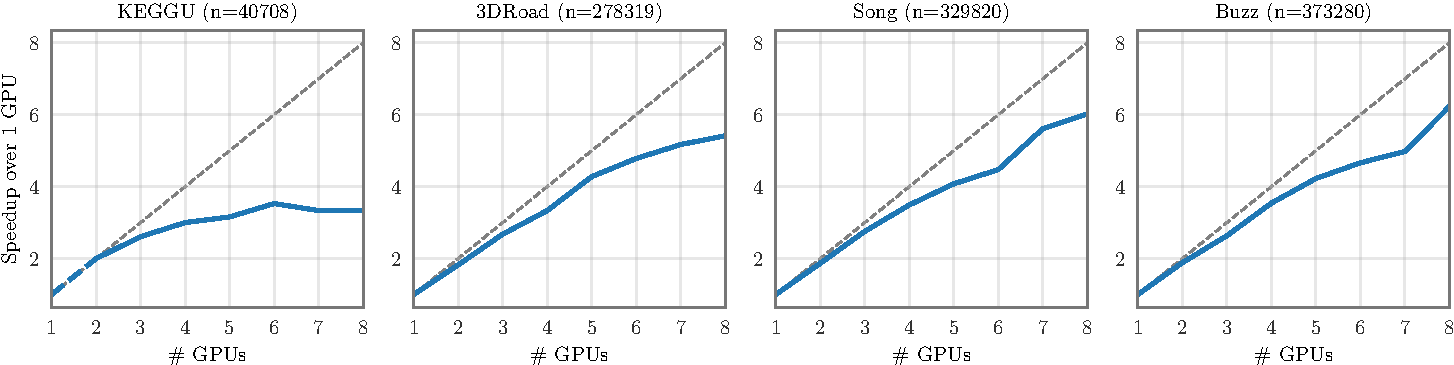
\includegraphics[width=\linewidth]{figures/gpu_speedup.pdf}
  \caption{
    Training speedup from using additional GPUs at training time.
    Since our exact GPs use matrix-multiplication based inference, they achieve a near linear speedup with more computing resources on large datasets.
  }
  \label{fig:gpu_speedup}
\end{figure*}


\paragraph{Training acceleration with multiple GPUs.}
Because we use matrix-multiplication-based approaches to train exact GPs, the computations can be easily parallelized and distributed.
Moreover, matrix multiplication is one of the most commonly distributed routines, so parallelized GP implementations can be built using readily-available routines in libraries like PyTorch \citep{paszke2017automatic}.
\autoref{fig:gpu_speedup} plots the speedup as more GPUs are used for training on the KEGGU, 3DRoad, Song, and Buzz datasets.
Each of these datasets achieve a nearly linear speedup when adding up to 4 GPUs.
The speedup is more pronounced for the two large datasets (3DRoad and Song) that require kernel partitioning.
The training time can be further improved by using more GPUs to reduce the number of kernel partitions.

\paragraph{Prediction time.}
Although exact GPs take longer to train, we find that \emph{their speed is comparable to approximate methods at test time.}
After training various GPs, we follow the common practice of precomputing the work required for GP predictions \citep{pleiss2018constant}.

\autoref{tab:large_exact_gp_timings} displays the time to compute $1,\!000$ predictive means and variances at test time before and after precomputation.
All predictions are made on one NVIDIA RTX 2080 Ti GPU. We see exact GPs take \emph{less than a second for all predictions} across all
dataset sizes used.
%
\subsection{Ablation Studies}
\begin{figure}[!t]
  \centering
  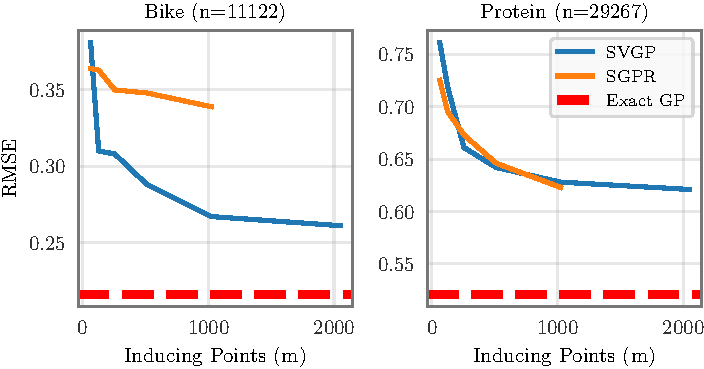
\includegraphics[width=0.8\linewidth]{figures/inducing_points.pdf}
  \caption{
    Error of SVGP and SGPR methods as a function of the number of inducing points
    ($m$).  Both methods scale cubically with $m$.
    We were unable to run SGPR with more than $1,\!024$ inducing points on a single GPU.
    Exact GPs have lower error than both methods.
  }
  \label{fig:num_inducing_points}
\end{figure}
With our method, we can better understand how exact GPs and approximate GPs scale to datasets with $n\gg 10^4$.
Here, we demonstrate how the amount of data affects exact GP performance, and
how the number of inducing points affects the performance of approximate GPs.
\begin{figure*}[t!]
  \centering
  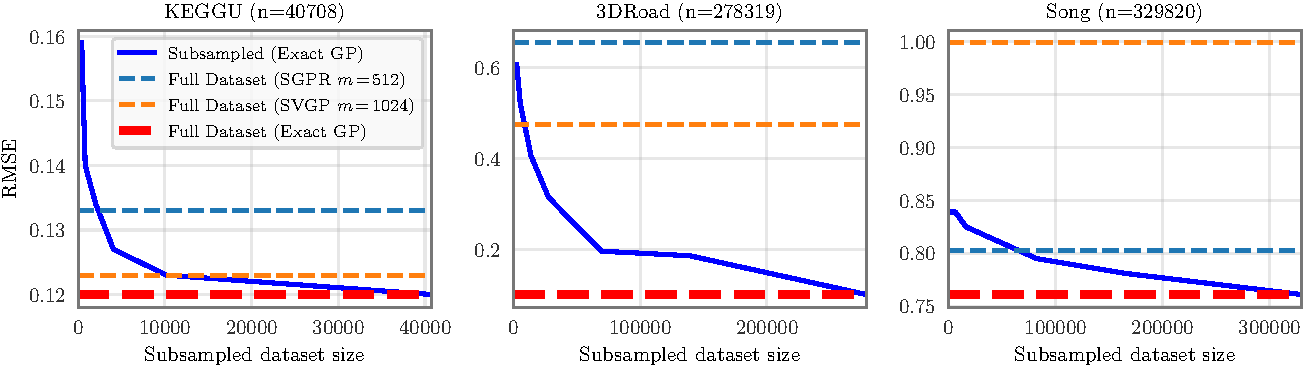
\includegraphics[width=\linewidth]{figures/subsampling.pdf}
  \caption{
    Test root-mean-square error (RMSE) as a function of subsampled dataset size (lower is better).
    Subsampled exact GPs outperform approximate GPs even with a quarter of the training set.
    Exact GP error continues to decrease as data is added until the full dataset is used.
  }
  \label{fig:subsampling_results}
\end{figure*}

\paragraph{Do GPs need the entire dataset?}
As a non-parametric model, Gaussian processes naturally adapt to the amount of training
data available \citep{wilsongpatt}. \autoref{fig:subsampling_results} shows an increase in accuracy as we increase the amount
of training data on the KEGGU, 3DRoad, and Song datasets. For each dataset, we
subsample a fraction of the training data and plot the resulting root-mean-square
error on the test-set as a function of subsampled training set size. We use the
same 1/3 holdout of the full dataset to test in each case.
As expected, the test RMSE decreases monotonically as we increase the subsample size.
\autoref{fig:subsampling_results} also shows the
performance of exact GP, SGPR, and SVGP trained on the entire training set.
Strikingly, in all three cases, \textit{an exact GP with less than a quarter of
the training data outperformed approximate GPs trained on the entire
training set}. Furthermore, test error continues to decrease with each addition of training data.

\paragraph{Would more inducing points help?}
The results in \cref{tab:large_exact_gp_results} naturally raise the question: ``can approximate models with more inducing
points recover the performance of exact methods?''
We plot test RMSE on two datasets, Bike and Protein, as a function of the number of inducing points in \autoref{fig:num_inducing_points}.
The test RMSE of both inducing point methods saturates on both datasets well above
the test RMSE of an exact GP.
Furthermore, we note that using $m$ inducing points introduces a $m \times m$
matrix and a $\bigo{nm^2 + m^3}$ time complexity
\cite{hensman2013gaussian,hensman2015scalable} which makes it
difficult to train SGPR with $m \gg 1024$ inducing points on
one GPU. It is possible to combine kernel partitioning with inducing-point methods to utilize even larger values of $m$.
However, as \autoref{fig:num_inducing_points} and \autoref{tab:large_exact_gp_results} show, it may be preferable
to use the extra computational resources to train an exact GP on more data rather than
to train an approximate GP with more inducing points.
%
